%%%%%%%%%%%%%%%%%%%%%%%%%%%%%%%%%%%%%%%%%
% Engineering Calculation Paper
% LaTeX Template
% Version 1.0 (20/1/13)
%
% This template has been downloaded from:
% http://www.LaTeXTemplates.com
%
% Original author:
% Dmitry Volynkin (dim_voly@yahoo.com.au)
%
% License:
% CC BY-NC-SA 3.0 (http://creativecommons.org/licenses/by-nc-sa/3.0/)
%
%%%%%%%%%%%%%%%%%%%%%%%%%%%%%%%%%%%%%%%%%

%----------------------------------------------------------------------------------------
%	PACKAGES AND OTHER DOCUMENT CONFIGURATIONS
%----------------------------------------------------------------------------------------

\documentclass[12pt,a4paper]{article} % Use A4 paper with a 12pt font size - different paper sizes will require manual recalculation of page margins and border positions
\usepackage[utf8]{inputenc}
\usepackage{marginnote} % Required for margin notes
\usepackage{wallpaper} % Required to set each page to have a background
\usepackage[francais]{babel}
%\usepackage{bclogo}
\usepackage{tikz}
\usetikzlibrary{shapes,snakes}
\usetikzlibrary{mindmap,trees}
\usepackage{lastpage} % Required to print the total number of pages
\usepackage[left=1.3cm,right=4.6cm,top=1.8cm,bottom=4.0cm,marginparwidth=3.4cm]{geometry} % Adjust page margins
\usepackage{amsmath} % Required for equation customization
\usepackage{amssymb} % Required to include mathematical symbols
\usepackage{xcolor} % Required to specify colors by name
\usepackage{enumerate}


\usepackage{tikz}
\usepackage[most]{tcolorbox}
\usepackage[pstricks]{bclogo}
\usepackage{pst-blur}

\usepackage{fancyhdr} % Required to customize headers
\setlength{\headheight}{80pt} % Increase the size of the header to accommodate meta-information
\pagestyle{fancy}\fancyhf{} % Use the custom header specified below
\renewcommand{\headrulewidth}{0pt} % Remove the default horizontal rule under the header

\setlength{\parindent}{0cm} % Remove paragraph indentation
\newcommand{\tab}{\hspace*{2em}} % Defines a new command for some horizontal space


%%%%%%%%%
%\renewcommand{\thesubsection}{[\Alph{section}](\alph{subsection})}
%%%%%%%%%

\newcommand\BackgroundStructure{ % Command to specify the background of each page
\setlength{\unitlength}{1mm} % Set the unit length to millimeters

\setlength\fboxsep{0mm} % Adjusts the distance between the frameboxes and the borderlines
\setlength\fboxrule{0.5mm} % Increase the thickness of the border line
\put(10, 10){\fcolorbox{black}{blue!1}{\framebox(155,247){}}} % Blue!1 , le numéro change la l'opacité de la couleur bleu
\put(165, 10){\fcolorbox{black}{blue!10}{\framebox(37,247){}}} % Margin box
\put(10, 262){\fcolorbox{black}{white!10}{\framebox(192, 25){}}} % Header box 160 et 263 pour régler la position du logo
\put(175, 263)    {
\includegraphics[height=23mm,keepaspectratio]{logo.png}} % Logo box - maximum height/width: 
}






%----------------------------------------------------------------------------------------
%	HEADER INFORMATION
%----------------------------------------------------------------------------------------
\fancyhead[L]{\begin{center}\textbf{DOSSIER RÉPONSE}\end{center} 
\begin{tabular}{l r | l r} 
\textbf{Sujet} & TP2.1 Désignation des outils de production  & TP noté $1^{er}$ semestre \\ 
\textbf{BTS} & CPRP 1 & \the\year-2023 & Page : \thepage/\pageref{LastPage} \\ 
\end{tabular}}
%----------------------------------------------------------------------------------------










\begin{document}


%%%%POUR FAIRE DES EXERCICES INDÉPENDAMMENT DES SECTIONS%%%%
%%%%%%%%%%%%%%%%%%%%%%%%%%%%%%%%%%%%%%%%%%%%%%%%%%%%%%%%%%%%%%%%%%%
\newcounter{exo}
\newenvironment{exo}{\stepcounter{exo}\vspace{0.5cm}{\bfseries Question \theexo\ :}}{\par\vspace{0.5cm}}
%%%%%%%%%%%%%%%%%%%%%%%%%%%%%%%%%%%%%%%%%%%%%%%%%%%%%%%%%%%%%%%%%%%%

\AddToShipoutPicture{\BackgroundStructure} % Set the background of each page to that specified above in the header information section
%----------------------------------------------------------------------------------------
%	DOCUMENT CONTENT
%----------------------------------------------------------------------------------------


\begin{tcolorbox}[colback=blue!5!white,colframe=black!75!black] 
Nom : \hspace{6,5cm} Nom : \\
Prénom : \hspace{6cm} Prénom :\\
\end{tcolorbox} \marginnote{\footnotesize{Clarté \&  propreté rédactionnelle $\pm{3}$ pts}}

TP noté sur 36,5 puis ramené sur 20.


\section{Introduction générale} 



\begin{exo} Le \textbf{VRAI ou FAUX} \end{exo}  \marginnote{2,5 points \\ 0,25/r}
\begin{enumerate}[1)]
    \item VRAI \tikzset{every picture/.style={line width=0.75pt}}         
\begin{tikzpicture}[x=0.75pt,y=0.75pt,yscale=-1,xscale=1]
%uncomment if require: \path (0,32); %set diagram left start at 0, and has height of 32
%Shape: Square [id:dp6719550419727234] 
\draw   (9,8) -- (24,8) -- (24,23) -- (9,23) -- cycle ;\end{tikzpicture} \hspace{3cm}   FAUX \begin{tikzpicture}[x=0.75pt,y=0.75pt,yscale=-1,xscale=1]
%uncomment if require: \path (0,32); %set diagram left start at 0, and has height of 32
%Shape: Square [id:dp6719550419727234] 
\draw   (9,8) -- (24,8) -- (24,23) -- (9,23) -- cycle ;\end{tikzpicture}
    \item VRAI \tikzset{every picture/.style={line width=0.75pt}}         
\begin{tikzpicture}[x=0.75pt,y=0.75pt,yscale=-1,xscale=1]
%uncomment if require: \path (0,32); %set diagram left start at 0, and has height of 32
%Shape: Square [id:dp6719550419727234] 
\draw   (9,8) -- (24,8) -- (24,23) -- (9,23) -- cycle ;\end{tikzpicture} \hspace{3cm}   FAUX \begin{tikzpicture}[x=0.75pt,y=0.75pt,yscale=-1,xscale=1]
%uncomment if require: \path (0,32); %set diagram left start at 0, and has height of 32
%Shape: Square [id:dp6719550419727234] 
\draw   (9,8) -- (24,8) -- (24,23) -- (9,23) -- cycle ;\end{tikzpicture}  
    \item VRAI \tikzset{every picture/.style={line width=0.75pt}}         
\begin{tikzpicture}[x=0.75pt,y=0.75pt,yscale=-1,xscale=1]
%uncomment if require: \path (0,32); %set diagram left start at 0, and has height of 32
%Shape: Square [id:dp6719550419727234] 
\draw   (9,8) -- (24,8) -- (24,23) -- (9,23) -- cycle ;\end{tikzpicture} \hspace{3cm}   FAUX \begin{tikzpicture}[x=0.75pt,y=0.75pt,yscale=-1,xscale=1]
%uncomment if require: \path (0,32); %set diagram left start at 0, and has height of 32
%Shape: Square [id:dp6719550419727234] 
\draw   (9,8) -- (24,8) -- (24,23) -- (9,23) -- cycle ;\end{tikzpicture}  
    \item VRAI \tikzset{every picture/.style={line width=0.75pt}}         
\begin{tikzpicture}[x=0.75pt,y=0.75pt,yscale=-1,xscale=1]
%uncomment if require: \path (0,32); %set diagram left start at 0, and has height of 32
%Shape: Square [id:dp6719550419727234] 
\draw   (9,8) -- (24,8) -- (24,23) -- (9,23) -- cycle ;\end{tikzpicture} \hspace{3cm}   FAUX \begin{tikzpicture}[x=0.75pt,y=0.75pt,yscale=-1,xscale=1]
%uncomment if require: \path (0,32); %set diagram left start at 0, and has height of 32
%Shape: Square [id:dp6719550419727234] 
\draw   (9,8) -- (24,8) -- (24,23) -- (9,23) -- cycle ;\end{tikzpicture}  
    \item VRAI \tikzset{every picture/.style={line width=0.75pt}}         
\begin{tikzpicture}[x=0.75pt,y=0.75pt,yscale=-1,xscale=1]
%uncomment if require: \path (0,32); %set diagram left start at 0, and has height of 32
%Shape: Square [id:dp6719550419727234] 
\draw   (9,8) -- (24,8) -- (24,23) -- (9,23) -- cycle ;\end{tikzpicture} \hspace{3cm}   FAUX \begin{tikzpicture}[x=0.75pt,y=0.75pt,yscale=-1,xscale=1]
%uncomment if require: \path (0,32); %set diagram left start at 0, and has height of 32
%Shape: Square [id:dp6719550419727234] 
\draw   (9,8) -- (24,8) -- (24,23) -- (9,23) -- cycle ;\end{tikzpicture}  
    \item VRAI \tikzset{every picture/.style={line width=0.75pt}}         
\begin{tikzpicture}[x=0.75pt,y=0.75pt,yscale=-1,xscale=1]
%uncomment if require: \path (0,32); %set diagram left start at 0, and has height of 32
%Shape: Square [id:dp6719550419727234] 
\draw   (9,8) -- (24,8) -- (24,23) -- (9,23) -- cycle ;\end{tikzpicture} \hspace{3cm}   FAUX \begin{tikzpicture}[x=0.75pt,y=0.75pt,yscale=-1,xscale=1]
%uncomment if require: \path (0,32); %set diagram left start at 0, and has height of 32
%Shape: Square [id:dp6719550419727234] 
\draw   (9,8) -- (24,8) -- (24,23) -- (9,23) -- cycle ;\end{tikzpicture}  
    \item VRAI \tikzset{every picture/.style={line width=0.75pt}}         
\begin{tikzpicture}[x=0.75pt,y=0.75pt,yscale=-1,xscale=1]
%uncomment if require: \path (0,32); %set diagram left start at 0, and has height of 32
%Shape: Square [id:dp6719550419727234] 
\draw   (9,8) -- (24,8) -- (24,23) -- (9,23) -- cycle ;\end{tikzpicture} \hspace{3cm}   FAUX \begin{tikzpicture}[x=0.75pt,y=0.75pt,yscale=-1,xscale=1]
%uncomment if require: \path (0,32); %set diagram left start at 0, and has height of 32
%Shape: Square [id:dp6719550419727234] 
\draw   (9,8) -- (24,8) -- (24,23) -- (9,23) -- cycle ;\end{tikzpicture}  
    \item VRAI \tikzset{every picture/.style={line width=0.75pt}}         
\begin{tikzpicture}[x=0.75pt,y=0.75pt,yscale=-1,xscale=1]
%uncomment if require: \path (0,32); %set diagram left start at 0, and has height of 32
%Shape: Square [id:dp6719550419727234] 
\draw   (9,8) -- (24,8) -- (24,23) -- (9,23) -- cycle ;\end{tikzpicture} \hspace{3cm}   FAUX \begin{tikzpicture}[x=0.75pt,y=0.75pt,yscale=-1,xscale=1]
%uncomment if require: \path (0,32); %set diagram left start at 0, and has height of 32
%Shape: Square [id:dp6719550419727234] 
\draw   (9,8) -- (24,8) -- (24,23) -- (9,23) -- cycle ;\end{tikzpicture}  
    \item VRAI \tikzset{every picture/.style={line width=0.75pt}}         
\begin{tikzpicture}[x=0.75pt,y=0.75pt,yscale=-1,xscale=1]
%uncomment if require: \path (0,32); %set diagram left start at 0, and has height of 32
%Shape: Square [id:dp6719550419727234] 
\draw   (9,8) -- (24,8) -- (24,23) -- (9,23) -- cycle ;\end{tikzpicture} \hspace{3cm}   FAUX \begin{tikzpicture}[x=0.75pt,y=0.75pt,yscale=-1,xscale=1]
%uncomment if require: \path (0,32); %set diagram left start at 0, and has height of 32
%Shape: Square [id:dp6719550419727234] 
\draw   (9,8) -- (24,8) -- (24,23) -- (9,23) -- cycle ;\end{tikzpicture}  
    \item VRAI \tikzset{every picture/.style={line width=0.75pt}}         
\begin{tikzpicture}[x=0.75pt,y=0.75pt,yscale=-1,xscale=1]
%uncomment if require: \path (0,32); %set diagram left start at 0, and has height of 32
%Shape: Square [id:dp6719550419727234] 
\draw   (9,8) -- (24,8) -- (24,23) -- (9,23) -- cycle ;\end{tikzpicture} \hspace{3cm}   FAUX \begin{tikzpicture}[x=0.75pt,y=0.75pt,yscale=-1,xscale=1]
%uncomment if require: \path (0,32); %set diagram left start at 0, and has height of 32
%Shape: Square [id:dp6719550419727234] 
\draw   (9,8) -- (24,8) -- (24,23) -- (9,23) -- cycle ;\end{tikzpicture}  
    
    
\end{enumerate}


\begin{exo} Quelle est la première donnée d'entrée dont nous partons toujours pour commencer notre conception de processus ?\end{exo} \marginnote{0,5 pt}

\begin{tikzpicture}
\draw (0,0) -- (0,3) ;
\draw (0,3) -- (15,3) ;
\draw (15,3) -- (15,0) ;
\draw (15,0) -- (0,0) ;
\end{tikzpicture}

\newpage  %%%%%%%%%%%%%%%%%%%%%%%%%%

\begin{exo} A partir de la pièce de la figure ci-dessous, indiquez la matière, la quantité et le type de norme utilisé (Européenne, américaine).\end{exo}  
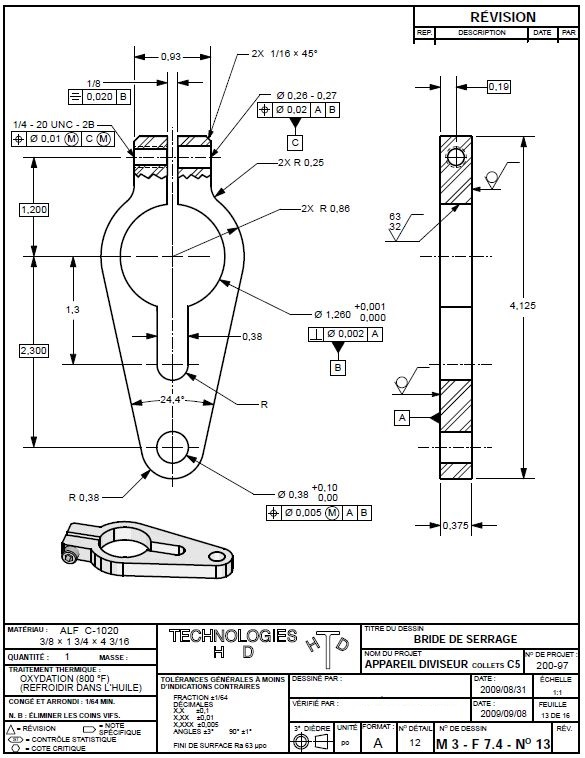
\includegraphics[scale=0.75]{dessin1.JPG}


 \marginnote{0,25 pt}
\begin{tikzpicture}
\draw (0,0) -- (0,2) ;
\draw (0,2) -- (15,2) ;
\draw (15,2) -- (15,0) ;
\draw (15,0) -- (0,0) ;
\draw (0.2,1.9) node [anchor=north west][inner sep=0.75pt]   [align=left] {MATIÈRE};
\end{tikzpicture}


\marginnote{0,25 pt}
\begin{tikzpicture}
\draw (0,0) -- (0,2) ;
\draw (0,2) -- (15,2) ;
\draw (15,2) -- (15,0) ;
\draw (15,0) -- (0,0) ;
\draw (0.2,1.9) node [anchor=north west][inner sep=0.75pt]   [align=left] {QUANTITÉ};
\end{tikzpicture}



\marginnote{0,25 pt}
\begin{tikzpicture}
\draw (0,0) -- (0,2) ;
\draw (0,2) -- (15,2) ;
\draw (15,2) -- (15,0) ;
\draw (15,0) -- (0,0) ;
\draw (0.2,1.9) node [anchor=north west][inner sep=0.75pt]   [align=left] {NORME};
\end{tikzpicture}  

\newpage


\begin{exo} A partir de la pièce de la Figure du dessus, et d'après vos recherche, quel est le type de traitement utilisé sur la pièce, et quel est son intérêt ? \end{exo}

\marginnote{0,25 pt}
\begin{tikzpicture}
\draw (0,0) -- (0,2) ;
\draw (0,2) -- (15,2) ;
\draw (15,2) -- (15,0) ;
\draw (15,0) -- (0,0) ;
\draw (0.2,1.9) node [anchor=north west][inner sep=0.75pt]   [align=left] {Type de traitement utilisé :};
\end{tikzpicture} 


\marginnote{1 pt}
\begin{tikzpicture}
\draw (0,0) -- (0,3) ;
\draw (0,3) -- (15,3) ;
\draw (15,3) -- (15,0) ;
\draw (15,0) -- (0,0) ;
\draw (0.2,2.9) node [anchor=north west][inner sep=0.75pt]   [align=left] {Intérêt du traitement :};
\end{tikzpicture}


\section{Quelles sont les différentes opérations d'usinage}
\subsection{Génération de surfaces}


\begin{exo} Quelle est la génératrice qui engendre un \textbf{cylindre} ? Quel est l'\textbf{axe de rotation} pour l'engendrer ? Vous ferez un schéma pour expliquez votre solution.\end{exo}



\tikzset{every picture/.style={line width=0.75pt}} %set default line width to 0.75pt        
\marginnote{1 pt}
\begin{tikzpicture}[x=0.75pt,y=0.75pt,yscale=-1,xscale=1]
%uncomment if require: \path (0,181); %set diagram left start at 0, and has height of 181

%Shape: Rectangle [id:dp49817033653449805] 
\draw   (25,16) -- (584.5,16) -- (584.5,250) -- (25,250) -- cycle ;
%Straight Lines [id:da033773758754015226] 
\draw    (315.75,16) -- (315.75,250) ;

% Text Node
\draw (40.75,26) node [anchor=north west][inner sep=0.75pt]   [align=left] {Réponse :};
% Text Node
\draw (321.75,25) node [anchor=north west][inner sep=0.75pt]   [align=left] {Schéma :};
\end{tikzpicture}

\newpage


\begin{exo} Quelle est la génératrice qui engendre un \textbf{cône} ? Quel est l'\textbf{axe de rotation} pour l'engendrer ? Vous ferez un schéma pour expliquez votre solution.\end{exo}




\tikzset{every picture/.style={line width=0.75pt}} %set default line width to 0.75pt        
\marginnote{1 pt}
\begin{tikzpicture}[x=0.75pt,y=0.75pt,yscale=-1,xscale=1]
%uncomment if require: \path (0,181); %set diagram left start at 0, and has height of 181

%Shape: Rectangle [id:dp49817033653449805] 
\draw   (25,16) -- (584.5,16) -- (584.5,250) -- (25,250) -- cycle ;
%Straight Lines [id:da033773758754015226] 
\draw    (315.75,16) -- (315.75,250) ;

% Text Node
\draw (40.75,26) node [anchor=north west][inner sep=0.75pt]   [align=left] {Réponse :};
% Text Node
\draw (321.75,25) node [anchor=north west][inner sep=0.75pt]   [align=left] {Schéma :};

\end{tikzpicture}

\newpage

\subsection{Le fraisage}
\begin{exo} Complétez le tableau d'opération d'usinage en tournage sur le document réponse. Vous devrez renseigner le ou les noms des opérations, la ou les formes/surfaces engendrées et enfin le ou les noms complets des outils.  \end{exo}
\marginnote{0,25 pt / réponse \\ = 3,75 pts}
\begin{center}
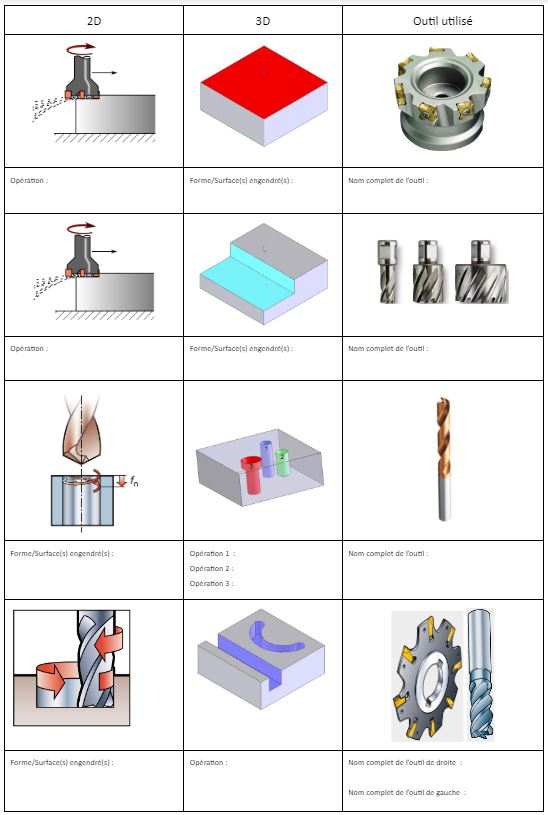
\includegraphics[scale=0.85]{FR1.JPG}
\end{center}

\newpage

\subsection{Le tournage}
\begin{exo} Complétez le tableau d'opération d'usinage en fraisage sur le document réponse. Vous devrez renseigner le ou les noms des opérations, la ou les formes/surfaces engendrées et enfin le ou les noms complet des outils.  \end{exo}
\marginnote{0,25 pt / réponse \\ = 3,25 pts}
\begin{center}
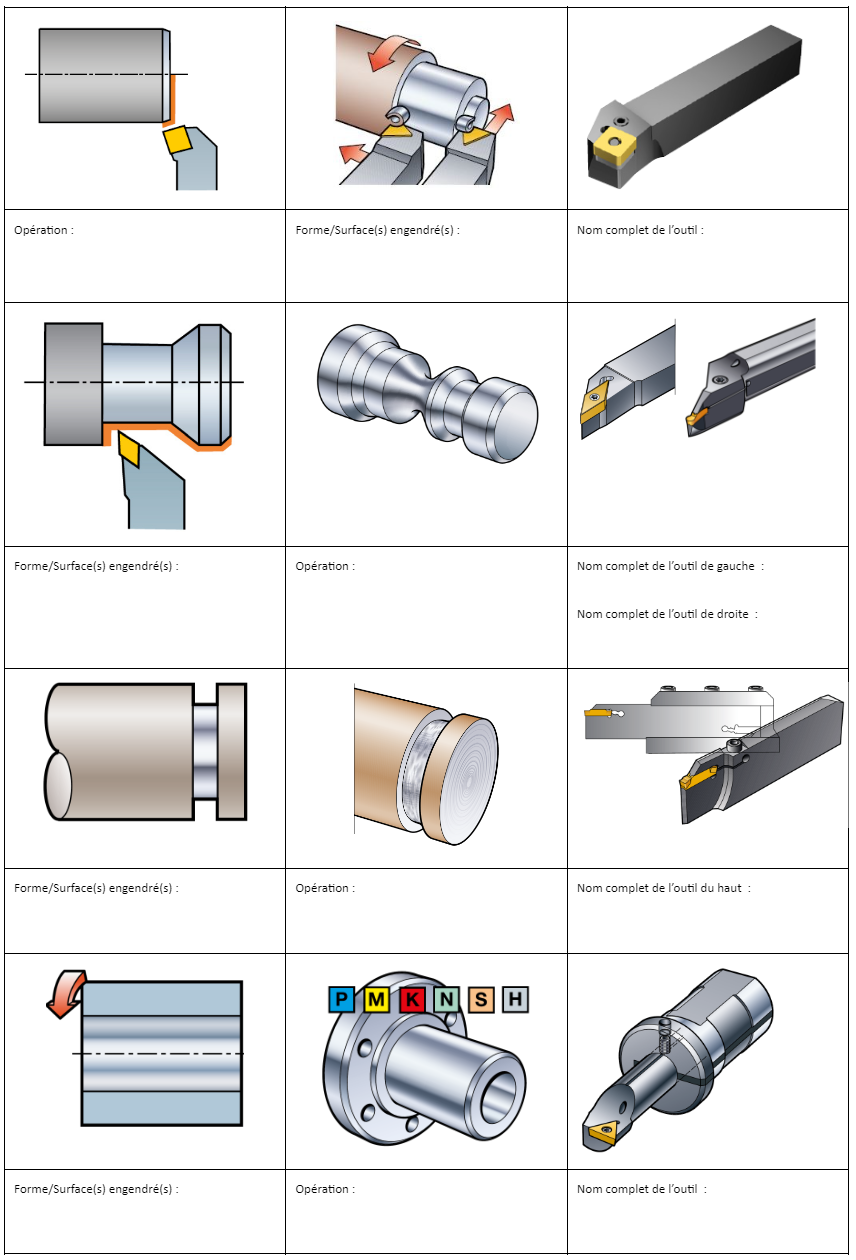
\includegraphics[scale=1.1]{TR1.png}
\end{center}



\section{Désignation des outils}
\subsection{Introduction}

\begin{exo} Quelles peuvent être les contraintes extérieures qui agissent sur le systèmes d'attache lors d'un usinage ? Vous citerez au moins 4 contraintes.\end{exo}

\marginnote{0,25 pt}
\begin{tikzpicture}
\draw (0,0) -- (0,2) ;
\draw (0,2) -- (15,2) ;
\draw (15,2) -- (15,0) ;
\draw (15,0) -- (0,0) ;
\draw (0.2,1.9) node [anchor=north west][inner sep=0.75pt]   [align=left] {1};
\end{tikzpicture}


\marginnote{0,25 pt}
\begin{tikzpicture}
\draw (0,0) -- (0,2) ;
\draw (0,2) -- (15,2) ;
\draw (15,2) -- (15,0) ;
\draw (15,0) -- (0,0) ;
\draw (0.2,1.9) node [anchor=north west][inner sep=0.75pt]   [align=left] {2};
\end{tikzpicture}



\marginnote{0,25 pt}
\begin{tikzpicture}
\draw (0,0) -- (0,2) ;
\draw (0,2) -- (15,2) ;
\draw (15,2) -- (15,0) ;
\draw (15,0) -- (0,0) ;
\draw (0.2,1.9) node [anchor=north west][inner sep=0.75pt]   [align=left] {3};
\end{tikzpicture}  

\marginnote{0,25 pt}
\begin{tikzpicture}
\draw (0,0) -- (0,2) ;
\draw (0,2) -- (15,2) ;
\draw (15,2) -- (15,0) ;
\draw (15,0) -- (0,0) ;
\draw (0.2,1.9) node [anchor=north west][inner sep=0.75pt]   [align=left] {4};
\end{tikzpicture}  



\begin{exo} Quelles doivent être les caractéristiques principales des broches d'attaches ? Vous citerez au moins 3 caractéristiques.\end{exo}


\marginnote{0,25 pt}
\begin{tikzpicture}
\draw (0,0) -- (0,2) ;
\draw (0,2) -- (15,2) ;
\draw (15,2) -- (15,0) ;
\draw (15,0) -- (0,0) ;
\draw (0.2,1.9) node [anchor=north west][inner sep=0.75pt]   [align=left] {1};
\end{tikzpicture}


\marginnote{0,25 pt}
\begin{tikzpicture}
\draw (0,0) -- (0,2) ;
\draw (0,2) -- (15,2) ;
\draw (15,2) -- (15,0) ;
\draw (15,0) -- (0,0) ;
\draw (0.2,1.9) node [anchor=north west][inner sep=0.75pt]   [align=left] {2};
\end{tikzpicture}



\marginnote{0,25 pt}
\begin{tikzpicture}
\draw (0,0) -- (0,2) ;
\draw (0,2) -- (15,2) ;
\draw (15,2) -- (15,0) ;
\draw (15,0) -- (0,0) ;
\draw (0.2,1.9) node [anchor=north west][inner sep=0.75pt]   [align=left] {3};
\end{tikzpicture}  


\newpage

\begin{exo} A l’aide du graphique, \textbf{justifiez} quelle est l’attache avec la meilleure transmission du couple pour les essais effectués. \end{exo}

\begin{minipage}{.55\linewidth}
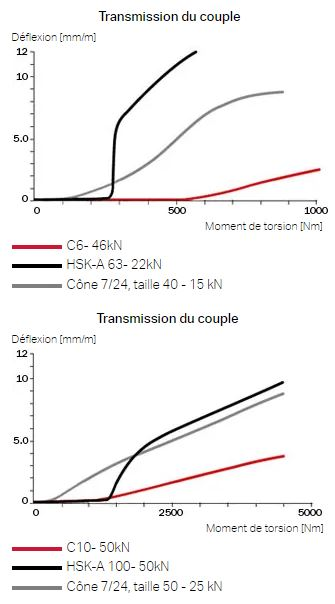
\includegraphics[scale=0.8]{T1.JPG}
\end{minipage}
\begin{minipage}{.44\linewidth}
\marginnote{1,25 pt}
\begin{tikzpicture}
\draw (0,0) -- (0,12) ;
\draw (0,12) -- (6,12) ;
\draw (6,12) -- (6,0) ;
\draw (6,0) -- (0,0) ;
\draw (0.2,11.9) node [anchor=north west][inner sep=0.75pt]   [align=left] {Justification :};
\end{tikzpicture}  
\end{minipage}

\begin{tikzpicture}
\draw (0,0) -- (0,4) ;
\draw (0,4) -- (15,4) ;
\draw (15,4) -- (15,0) ;
\draw (15,0) -- (0,0) ;
\draw (0.2,3.9) node [anchor=north west][inner sep=0.75pt]   [align=left] {Espace libre};
\end{tikzpicture}  

\newpage


\subsection{Les outils en tournage}

\begin{exo} Nommer les différents  éléments de l’outil d’usinage à l'aide des mots
indiqués. \end{exo}
\marginnote{0,25 pt/réponse \\ = 1,5 pt}
\begin{minipage}{.55\linewidth}
\begin{itemize}
    \item Porte-outil;
    \item Sortie huile de coupe
    \item Liaison vis sans fin
\end{itemize} 
\end{minipage}
\begin{minipage}{.44\linewidth}
\begin{itemize}
    \item Plaquettes
    \item Cales
    \item Porte plaquette
\end{itemize} 
\end{minipage}
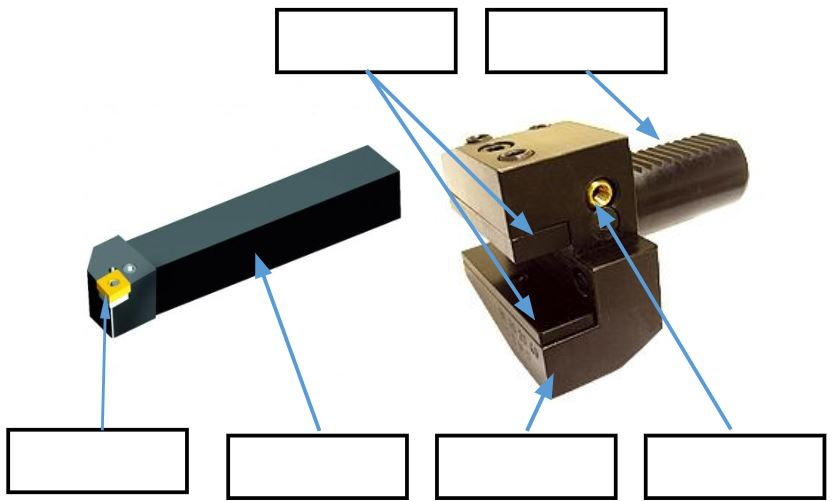
\includegraphics[scale=0.65]{PP1.JPG}

\newpage

\subsection{Les outils en fraisage}

\begin{exo} Nommez les différents éléments de l’outil d’usinage figure à l'aide des mots
indiques dans le dossier réponse. \end{exo}


\begin{minipage}{.55\linewidth}
\begin{itemize}
    \item  \begin{tikzpicture} \draw (0,0) circle (0.5) ; \end{tikzpicture} Porte-outil;
    \item  \begin{tikzpicture} \draw (0,0) circle (0.5) ; \end{tikzpicture} Foret monobloc;
    \item  \begin{tikzpicture} \draw (0,0) circle (0.5) ; \end{tikzpicture} Liaison vis sans fin;
    \item  \begin{tikzpicture} \draw (0,0) circle (0.5) ; \end{tikzpicture} Clavette d'entraînement (transmission du couple);
\end{itemize} 
\end{minipage}
\begin{minipage}{.44\linewidth}
\begin{itemize}
    \item  \begin{tikzpicture} \draw (0,0) circle (0.5) ; \end{tikzpicture} Outil;
    \item  \begin{tikzpicture} \draw (0,0) circle (0.5) ; \end{tikzpicture} Dispositif de serrage;
    \item  \begin{tikzpicture} \draw (0,0) circle (0.5) ; \end{tikzpicture} Magasin outil / Tourelle;
\end{itemize} 
\end{minipage}


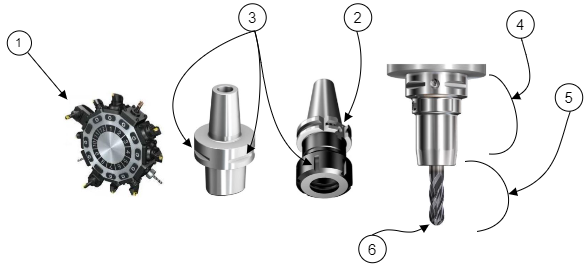
\includegraphics[scale=0.95]{FF1.png}

 

\newpage

\subsection{Lubrification}

\begin{exo} Quels peuvent être les deux intérêts principaux de l'utilisation d'une lubrification interne ou externe ? Comparez les deux technologies.\end{exo}
\begin{center}
    \textbf{Lubrification EXTERNE}
\end{center}

\marginnote{1,25 pt}
\begin{tikzpicture}
\draw (0,0) -- (0,5) ;
\draw (0,5) -- (15,5) ;
\draw (7.5,5) -- (7.5,0) ;
\draw (15,5) -- (15,0) ;
\draw (15,0) -- (0,0) ;
\draw (0.2,4.9) node [anchor=north west][inner sep=0.75pt]   [align=left] {Avantages};
\draw (7.7,4.9) node [anchor=north west][inner sep=0.75pt]   [align=left] {Inconvénients};
\end{tikzpicture}  



\begin{center}
    \textbf{Lubrification INTERNE}
\end{center}

\marginnote{1,25 pt}
\begin{tikzpicture}
\draw (0,0) -- (0,5) ;
\draw (0,5) -- (15,5) ;
\draw (7.5,5) -- (7.5,0) ;
\draw (15,5) -- (15,0) ;
\draw (15,0) -- (0,0) ;
\draw (0.2,4.9) node [anchor=north west][inner sep=0.75pt]   [align=left] {Avantages};
\draw (7.7,4.9) node [anchor=north west][inner sep=0.75pt]   [align=left] {Inconvénients};
\end{tikzpicture}  










%%%%%%%%%%%%%%%%%%%%%%%%%%%%%%%%%%%%%%%%%%%%%%%%%%%%%%%%%%%%%%%%%%%%%%%%%%%%
\begin{figure}[h]
\centering

\includegraphics[scale=0.75]{logo.png}
\caption{Complétez directement sur le sujet, l'opération, la forme générée et le nom de l'outil, en vous aidant des dessins du schéma.}
\label{exo1}
\end{figure}
%%%%%%%%%%%%%%%%%%%%%%%%%%%%%%%%%%%%%%%%%%%%%%%%%%%%%%%%%%%%%%%%%%%%%%%%%%%%%%



\begin{tikzpicture}
\draw (0,0) -- (0,7) ;
\draw (0,7) -- (15,7) ;
\draw (15,7) -- (15,0) ;
\draw (15,0) -- (0,0) ;
\end{tikzpicture}


%----------------------------------------------------------------------------------------

\end{document}